\documentclass[a4paper,12pt]{article}

\usepackage[utf8]{inputenc}%рассказываем компилятору, какая кодировка документа
\usepackage[russian]{babel}%подключаем Русский язык

\usepackage[left=2cm,right=1cm,top=2cm,bottom=2cm]{geometry}%отступы страницы

\usepackage{indentfirst}%красная строка после заголовков
\usepackage{graphicx,xcolor}%вставка картинок и графики


\begin{document}
	
\section{Отчет по OSCP}
\subsection {Введение}
Данный пейпер посвящен подробному описанию по поиску и эксплуатированию уязвимостей в сети при прохождении сертификации OSCP (Offensive Security Certified Pentester)


Весь нижеуказанный материал предоставлен исключительно в ознакомительных и целях. Автор данного текста не несет ответственности за последствия.
\subsection{Исходные данные}
Имеется подсеть в диапазоне от 10.11.1.1 по 10.11.1.255. Ничего об этой сети более не известно. Сеть является vpn и эмулирует полностью работу небольшой компании. Сеть представляет из себя набор подсетей, для доступа к которым необходимо пробрасывать тунели со взломанных машин. 

\begin{figure}[h!]
	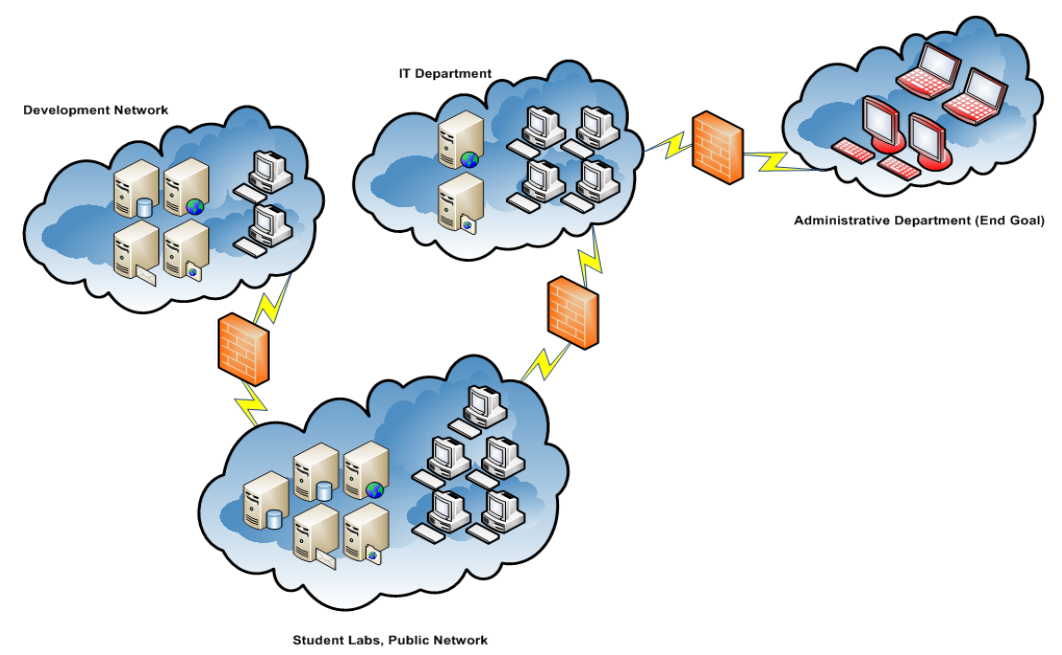
\includegraphics[width=\linewidth]{net.png}
	\caption{Макет сети лаборатории.}
	\label{fig:boat1}
\end{figure}

Задача: собрать как можно больше данных о сети и выбрать первую цель для атаки. 


\section{Базовый сбор информации о сети}
Здесь я опущу бОльшую часть подробностей. Будем использовать классический ping sweep для поиска в сети живых машин. Можно было бы написать свой скрипт на bash, но проще воспользоваться уже готовым вариантом в составе софта nmap. Собственно, просканируем сеть и запишем полученные данные в hosts.txt
\begin{figure}[h!]
	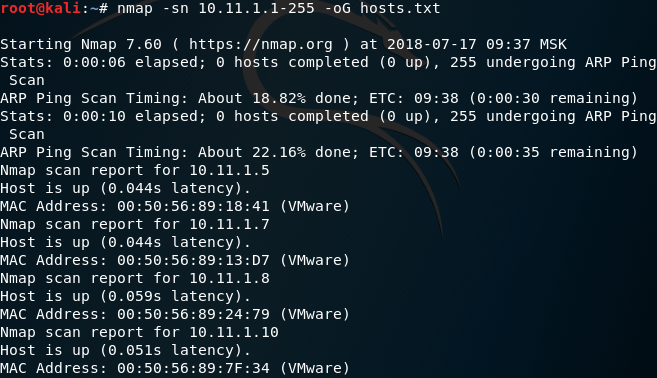
\includegraphics[width=\linewidth]{nmap_start_1.png}
	\caption{Сканируем всю подсеть на наличие "живых" машин.}
	\label{fig:boat1}
\end{figure}

Отлично! Теперь посмотрим, что у нас получилось. 
\newpage
\begin{figure}[h!]
	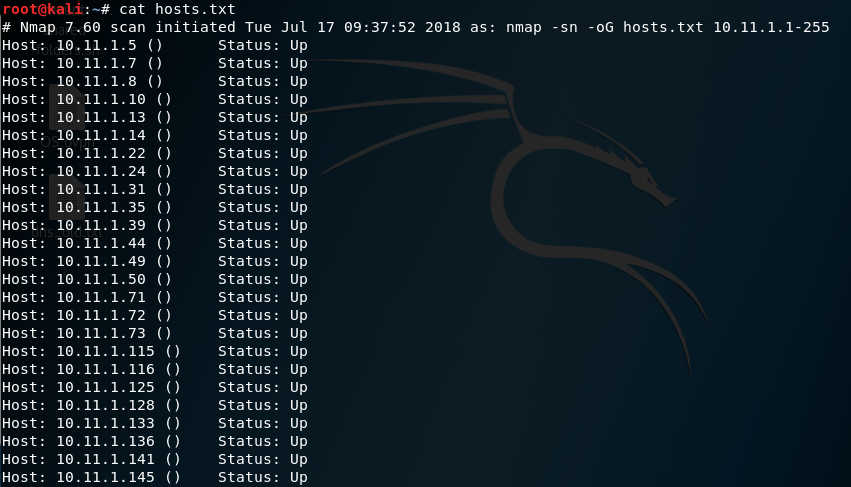
\includegraphics[width=\linewidth]{cat_hosts_2.png}
	\caption{Выводим полученный список "живых" машин.}
	\label{fig:boat2}
\end{figure}


Как видно, у нас теперь есть список живых машин, но он представлен не совсем в чистом виде. Попробуем написать маленький скриптик, чтобы список содержал только айпишники. 
\newpage
\begin{figure}[h!]
	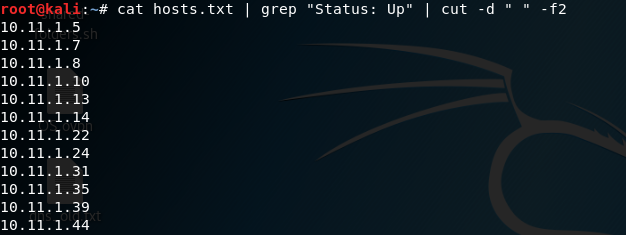
\includegraphics[width=\linewidth]{cat_cut_3.png}
	\caption{Получаем чистый список айпишников}
	\label{fig:boat3}
\end{figure}

Теперь этот список можно скармливать различным скриптам и программам. Попробуем получить названия машин в сети. Для этого напишем еще один простой bash-скрипт. 	


\begin{figure}[h!]
	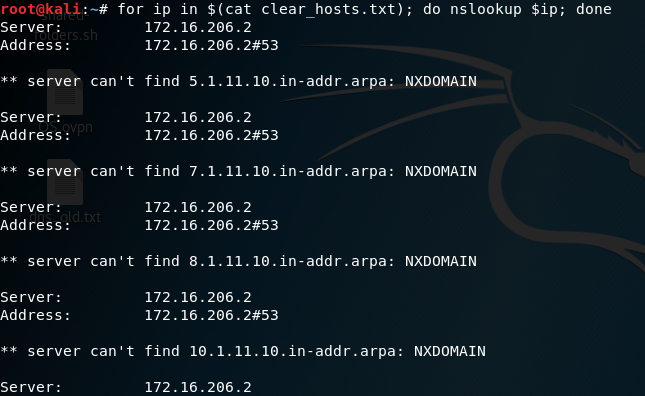
\includegraphics[width=\linewidth]{bad_nslookup_4.png}
	\caption{Пробуем получить названия машин в сети.}
	\label{fig:boat2}
\end{figure}

Как видим, названия получить не удается. Все дело в том, что названия машины в сети это информация типа CNAME, за которую отвечает DNS-сервер, а наш DNS-сервер из обычной сети понятия не имеет о том, что происходит в vpn.

Чтобы поправить ситуацию, нам необходимо найти DNS-сервер внтури нашей приватной сети(vpn) - вот он-то будет знать все о местных машинах. Этим и займемся:
Для начала немного о DNS. Его отличительная особенность - открытые порты 53 на tcp и udp. Поэтому просто сканируем сеть nmap'ом по 53ему порту.

\begin{figure}[h!]
	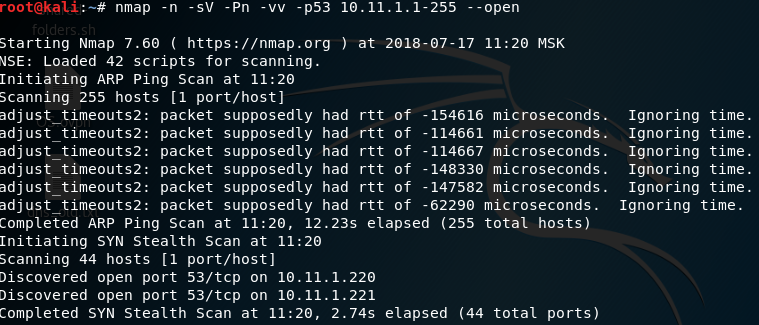
\includegraphics[width=\linewidth]{nmap_dns_search_6.png}
	\caption{Ищем DNS-server'ы.}
	\label{fig:boat2}
\end{figure}

Видим два айпишника с открытыми 53 портами... Попробуем узнать о них немного побольше.

\begin{figure}[h!]
	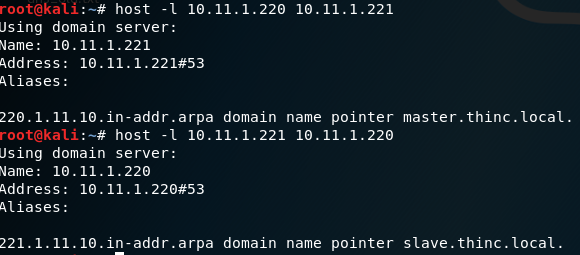
\includegraphics[width=\linewidth]{dns_master_slave_61.png}
	\caption{Получаем два DNS-сервера.}
	\label{fig:boat2}
\end{figure}

Ага...Два DNS-сервера. Один - мастер, второй - слейв. Отлично. Тепреь мы можем узнать у них информацию о других машинах в сети.
Для этого найдем конфиг, который отвечает за настройки DNS-сервера, который в данный момент наша система считает таковым и заменим в нем адрес на новый ip нашего DNS-master-сервера. (пиздец я криво пишу)
\newpage
\begin{figure}[h!]
	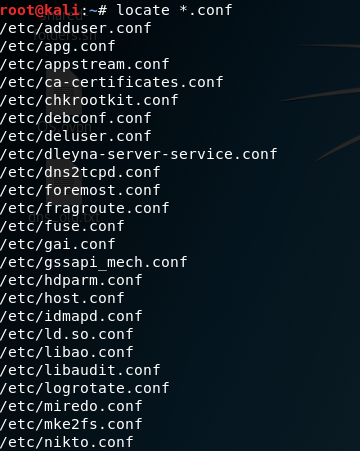
\includegraphics[width=\linewidth]{searching_for_conf_5.png}
	\caption{Ищем нужный конфиг.}
	\label{fig:boat4}
\end{figure}

\begin{figure}[h!]
	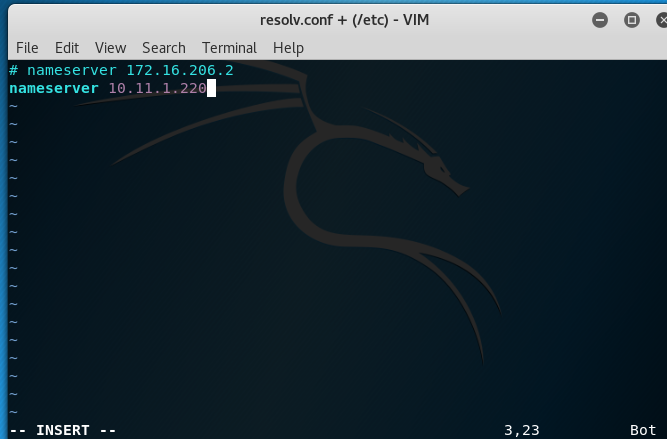
\includegraphics[width=\linewidth]{resolv_conf_dns_7.png}
	\caption{Комментируем старую строчку и подменяем DNS.}
	\label{fig:boat2}
\end{figure}

\newpage

Отлично! Теперь мы можем снова опросить теперь уже новый DNS-сервер о том, что он знает о машинах в текущей сети. Запускаем nslookup.

\begin{figure}[h!]
	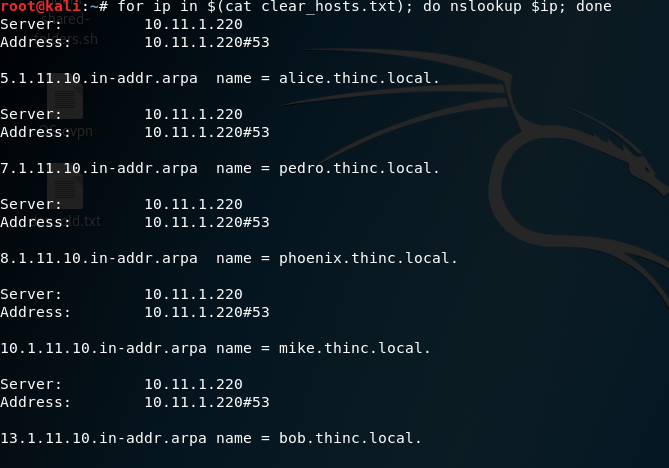
\includegraphics[width=\linewidth]{succes_nslookup_8.png}
	\caption{Получаем названия машин в сети.}
	\label{fig:boat2}
\end{figure}
\newpage
Вот и все. Теперь мы вычислили все живые машины в этой сети и даже получили их имена.


\section{APT Alpha}
Эта секция посвящена таргетированной атаке машины под ником Alpha, котоая имеет ip-адрес 10.11.1.71.




\end{document}
